\chapter{Gauss-Siedel, SOR \& LOR}


\section{Metodo di Gauss-Seidel}

Il metodo di Jacobi calcola il flusso in ogni nodo all'iterazione $m+1$ sulla base dei flussi ottenuti all'iterazione $m$. Tuttavia, quando si aggiorna il flusso nel nodo di coordinate $(i,j)$, i nodi con indici $i$ e $j$ minori sono già stati aggiornati.

Il metodo di Gauss-Seidel cerca di sfruttare immediatamente i flussi già aggiornati nell'iterazione corrente. Per fare ciò, si immagina di decomporre ulteriormente la matrice di iterazione di Jacobi $\mathbf{H}$ come segue:

\begin{equation*}
	\mathbf{H} = \mathbf{L} + \mathbf{U} \tag{1}
\end{equation*}

dove

\[
\mathbf{L} = \left[ \begin{array}{c c c c c}
	0 & 0 & 0 & \circ & 0 \\
	- \frac{a_{21}}{a_{22}} & 0 & 0 & \circ & 0 \\
	- \frac{a_{31}}{a_{33}} & - \frac{a_{32}}{a_{33}} & 0 & \circ & 0 \\
	\vdots & \vdots & \vdots & \ddots & \vdots \\
	- \frac{a_{n1}}{a_{nn}} & - \frac{a_{n2}}{a_{nn}} & - \frac{a_{n3}}{a_{nn}} & \circ & 0
\end{array} \right],
\quad
\mathbf{U} = \left[ \begin{array}{c c c c c}
	0 & - \frac{a_{12}}{a_{11}} & - \frac{a_{13}}{a_{11}} & \circ & - \frac{a_{1n}}{a_{11}} \\
	0 & 0 & - \frac{a_{23}}{a_{22}} & \circ & - \frac{a_{2n}}{a_{22}} \\
	0 & 0 & 0 & \circ & - \frac{a_{3n}}{a_{33}} \\
	\vdots & \vdots & \vdots & \ddots & \vdots \\
	0 & 0 & 0 & \circ & 0
\end{array} \right].
\]

L'equazione di iterazione assume la nuova forma:

\begin{equation*}
	\mathbf{\phi} = \mathbf{H} \mathbf{\phi} + \mathbf{q} 
	\qquad \Rightarrow \qquad \mathbf{\phi} = \mathbf{L} \mathbf{\phi} + \mathbf{U} \mathbf{\phi} + \mathbf{q} \tag{2}
\end{equation*}

che, scritta in termini di componenti,

\begin{equation}
	\phi_i = \sum_{j=1}^{i-1} l_{i,j} \phi_j + \sum_{j=i+1}^n u_{i,j} \phi_j + q_i \tag{3}
\end{equation}

permette di impostare il seguente schema iterativo:

\begin{equation}
	\mathbf{\phi}^{(m+1)} = \mathbf{L} \mathbf{\phi}^{(m+1)} + \mathbf{U} \mathbf{\phi}^{(m)} + \mathbf{q}. \tag{4}
\end{equation}

È un dato di fatto che i flussi nella prima somma dell'Eq.(3) appartengono a nodi che sono già stati aggiornati nel corso dell'iterazione $(m+1)$.

Partendo dall'Eq.(4), si ottiene:

\[ \begin{aligned}
\mathbf{\phi}^{(m+1)} &= \mathbf{L} \mathbf{\phi}^{(m+1)} + \mathbf{U} \mathbf{\phi}^{(m)} + \mathbf{q}\ \ ,\\
(\mathbf{I} - \mathbf{L}) \mathbf{\phi}^{(m+1)} &= \mathbf{U} \mathbf{\phi}^{(m)} + \mathbf{q}\ \ ,\\
\mathbf{\phi}^{(m+1)} &= (\mathbf{I} - \mathbf{L})^{-1} \mathbf{U} \mathbf{\phi}^{(m)} + (\mathbf{I} - \mathbf{L})^{-1} \mathbf{q}\ \ . 
\end{aligned}\]

La matrice di iterazione di Gauss-Seidel è quindi: $\boxed{\mathbf{H}_{GS} = (\mathbf{I} - \mathbf{L})^{-1} \mathbf{U}}$ .

È possibile dimostrare che il raggio spettrale di \(\mathbf{H}_{GS}\) è legato a quello della matrice di Jacobi \(\mathbf{H}_J\) dalla relazione:

\[
\boxed{\,\rho(\mathbf{H}_{GS}) = \left[ \rho(\mathbf{H}_J) \right]^2\,}\ \ \ . 
\]

\subsubsection{Velocità di convergenza}

Nel caso del metodo di Gauss-Seidel, la velocità asintotica di convergenza è data da:

\[
R_{\infty}^{GS}\ =\ -\,\ln \rho(\mathbf{H}_{GS})\ =\ -\,2\, \ln \rho(\mathbf{H}_J)\ =\ 2\, R_{\infty}^{J}, 
\]

dove \(R_{\infty}^{J}\) è la velocità asintotica di convergenza del metodo di Jacobi.

Di conseguenza, il metodo di Gauss-Seidel converge più rapidamente del metodo di Jacobi, richiedendo circa la metà delle iterazioni.

\subsubsection{Implementazione pratica del metodo di Gauss-Seidel}

\begin{multicols}{2}
Il calcolo del flusso in ogni nodo coinvolge sia i valori dell'iterazione precedente che quelli dell'iterazione corrente. Ad esempio come si vede in figura di fianco, quando si aggiorna il flusso del nodo 10, per i nodi 4 e 9 si utilizzano i valori già aggiornati nell'iterazione corrente, mentre per i nodi 11 e 16 si adottano quelli dell'iterazione precedente.

\begin{figure}[H]
	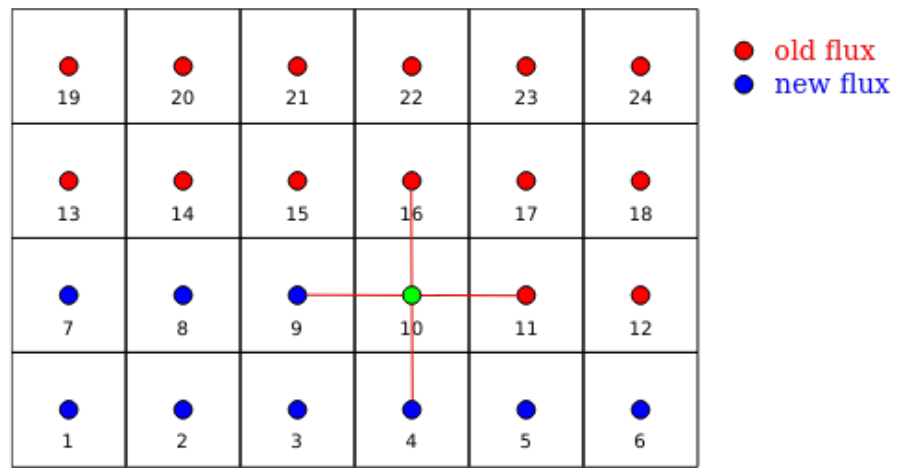
\includegraphics[width=7cm]{img/gs1.png}
	\label{gauss siedel 1}
	\caption{visualizzazione di Gauss-Siedel}
\end{figure}
\end{multicols}

Introducendo come per il metodo di Jacobi i coefficienti \(W_{i,j}\), \(E_{i,j}\), \(S_{i,j}\), \(N_{i,j}\) e il termine sorgente \(q_{i,j}\), lo schema iterativo può essere espresso come:

\[
\phi_{i,j}^{(m+1)} = W_{i,j} \phi_{i-1,j}^{(m+1)} + E_{i,j} \phi_{i+1,j}^{(m)} + S_{i,j} \phi_{i,j-1}^{(m+1)} + N_{i,j} \phi_{i,j+1}^{(m)} + q_{i,j}. \tag{9}
\]

\section{Metodo di Successive Overrelaxation (SOR)}

Il concetto di questo metodo è quello di estrapolare la previsione di Gauss-Seidel utilizzando un opportuno fattore di overrelaxation \(\omega > 1\). Partendo dalla stima di Gauss-Seidel all'iterazione \((m+1)\), Eq.(4), si sottrae \(\mathbf{\phi}^{(m)}\) da entrambi i membri:

\[
\mathbf{\phi}^{(m+1)} - \mathbf{\phi}^{(m)} = \mathbf{L} \mathbf{\phi}^{(m+1)} + (\mathbf{U} - \mathbf{I}) \mathbf{\phi}^{(m)} + \mathbf{q}\ \ . 
\]

Il flusso alla nuova iterazione \((m+1)\) viene quindi calcolato come:

\[
\mathbf{\phi}^{(m+1)} = \mathbf{\phi}^{(m)} + \omega \left[ \mathbf{\phi}^{(m+1)} - \mathbf{\phi}^{(m)} \right]_{GS},
\]

che, sostituendo l'Eq.(10), diventa:

\[
\mathbf{\phi}^{(m+1)} = \mathbf{\phi}^{(m)} + \omega \left[ \mathbf{L} \mathbf{\phi}^{(m+1)} + (\mathbf{U} - \mathbf{I}) \mathbf{\phi}^{(m)} + \mathbf{q} \right].
\]

Riorganizzando i termini, si ottiene:

\[
\mathbf{\phi}^{(m+1)} = \omega \mathbf{L} \mathbf{\phi}^{(m+1)} + \left[ (1 - \omega) \mathbf{I} + \omega \mathbf{U} \right] \mathbf{\phi}^{(m)} + \omega \mathbf{q}\ \ . 
\]

---

\subsection{Matrice di iterazione del metodo SOR}

Dall'Eq.(11) è possibile ricavare la matrice di iterazione dello schema iterativo SOR:

\[
\mathbf{\phi}^{(m+1)} = \left( \mathbf{I} - \omega \mathbf{L} \right)^{-1} \left[ (1 - \omega) \mathbf{I} + \omega \mathbf{U} \right] \mathbf{\phi}^{(m)} + \omega \left( \mathbf{I} - \omega \mathbf{L} \right)^{-1} \mathbf{q}\ \ . 
\]

La matrice di iterazione \(\mathbf{H}\) del metodo SOR è quindi:

\[
\mathbf{H} = \left( \mathbf{I} - \omega \mathbf{L} \right)^{-1} \left[ (1 - \omega) \mathbf{I} + \omega \mathbf{U} \right]\ \ . 
\]

È possibile dimostrare che esiste un valore ottimale di \(\omega\) che minimizza il raggio spettrale di \(\mathbf{H}\), dato da:

\[
\omega_{opt} = \frac{2}{1 + \sqrt{1 - \rho^2(\mathbf{H}_J)}}, \quad 1 \leq \omega_{opt} \leq 2\ \ . 
\]

Per calcolare \(\omega_{opt}\) è necessario conoscere il raggio spettrale della matrice di iterazione di Jacobi \(\mathbf{H}_J\).

\subsubsection{Stima del raggio spettrale di Jacobi}

Prima di avviare il processo iterativo SOR, è consigliabile eseguire un certo numero di iterazioni di Jacobi per ottenere una stima del suo raggio spettrale, \(\rho_{\mathbf{H}_J}\).

Consideriamo una matrice simmetrica \(\mathbf{H}_J\). Il vettore noto \(\mathbf{q}\) può essere espresso in termini degli autovettori di \(\mathbf{H}_J\) (che rappresentano una base ortogonale completa):

\[
\mathbf{q} = \sum_{h=1}^{n} q_h \mathbf{\varphi}_h\ \ . 
\]

Inoltre, ricordiamo che gli autovettori sono ortonormali, poiché \(\mathbf{U}^T \mathbf{U} = \mathbf{I}\).

---

\subsubsection{Derivazione della stima}

Si ha quindi:

\[
\begin{aligned}
	\left\| \mathbf{H}_J^m \mathbf{q} \right\|^2 &= \left( \mathbf{H}_J^m \mathbf{q}, \mathbf{H}_J^m \mathbf{q} \right) \\
	&= \left( \sum_{h=1}^{n} q_h \lambda_h^m \mathbf{\varphi}_h, \sum_{k=1}^{n} q_k \lambda_k^m \mathbf{\varphi}_k \right) \\
	&= \sum_{h=1}^{n} |q_h|^2 \lambda_h^{2m} \\
	&= \sum_{\substack{h: \\ |\lambda_h| = \rho_{\mathbf{H}_J}}}^n |q_h|^2 \rho_{\mathbf{H}_J}^{2m} + \sum_{\substack{h: \\ |\lambda_h| < \rho_{\mathbf{H}_J}}}^n |q_h|^2 \lambda_h^{2m} \\
	&= \rho_{\mathbf{H}_J}^{2m} \left[ \sum_{\substack{h: \\ |\lambda_h| = \rho_{\mathbf{H}_J}}}^n |q_h|^2 + \sum_{\substack{h: \\ |\lambda_h| < \rho_{\mathbf{H}_J}}}^n |q_h|^2 \frac{\lambda_h^{2m}}{\rho_{\mathbf{H}_J}^{2m}} \right]\ \ . 
\end{aligned}
\]

Consideriamo ora il seguente limite:

\[
\lim_{m \to \infty} \frac{\left\| \mathbf{H}_J^{m+1} \mathbf{q} \right\|^2}{\left\| \mathbf{H}_J^m \mathbf{q} \right\|^2}\ \ . 
\]

Dall'Eq.(16), per \(m \to \infty\), i rapporti nella sommatoria per \(h: |\lambda_h| < \rho_{\mathbf{H}_J}\) tenderanno tutti a zero, così che l'Eq.(17) si riduce a:

\[
\lim_{m \to \infty} \frac{\left\| \mathbf{H}_J^{m+1} \mathbf{q} \right\|^2}{\left\| \mathbf{H}_J^m \mathbf{q} \right\|^2} = \lim_{m \to \infty} \frac{\rho_{\mathbf{H}_J}^{2m+2}}{\rho_{\mathbf{H}_J}^{2m}} \frac{\sum_{h: |\lambda_h| = \rho_{\mathbf{H}_J}} |q_h|^2}{\sum_{h: |\lambda_h| = \rho_{\mathbf{H}_J}} |q_h|^2} = \rho_{\mathbf{H}_J}^2\ \ . 
\]

---

\subsection{Applicazione pratica}

In pratica, ricordando che:

\[
\mathbf{\phi}^{(m+1)} = \mathbf{H}_J \mathbf{\phi}^{(m)} + \mathbf{q} = \mathbf{H}_J^m \mathbf{q} + \mathbf{H}_J^{m-1} \mathbf{q} + \dots + \mathbf{q}\ \ , 
\]

si ha:

\[
\left\| \mathbf{\phi}^{(m+1)} - \mathbf{\phi}^{(m)} \right\| = \left\| \mathbf{H}_J^m \mathbf{q} \right\|\ \ . 
\]

Dall'Eq.(18), segue che:

\[
\lim_{m \to \infty} \frac{\left\| \mathbf{H}_J^{m+1} \mathbf{q} \right\|}{\left\| \mathbf{H}_J^m \mathbf{q} \right\|} = \lim_{m \to \infty} \frac{\left\| \mathbf{\phi}^{(m+2)} - \mathbf{\phi}^{(m+1)} \right\|}{\left\| \mathbf{\phi}^{(m+1)} - \mathbf{\phi}^{(m)} \right\|} = \rho_{\mathbf{H}_J}\ \ . 
\]

\begin{multicols}{2}
Pertanto, vengono eseguite diverse iterazioni di Jacobi fino a quando il rapporto \(\frac{\left\| \mathbf{\phi}^{(m+2)} - \mathbf{\phi}^{(m+1)} \right\|}{\left\| \mathbf{\phi}^{(m+1)} - \mathbf{\phi}^{(m)} \right\|}\) non viene considerato una stima sufficientemente accurata del raggio spettrale.

Inoltre si può mostrare che $\omega=\omega_{opt}$:
\[\rho_{\mathbf H_{SOR}}\ =\ \frac{2}{1+\sqrt{1-\rho^2_{\mathbf H_J}}}\,-\,1\]

\begin{figure}[H]
	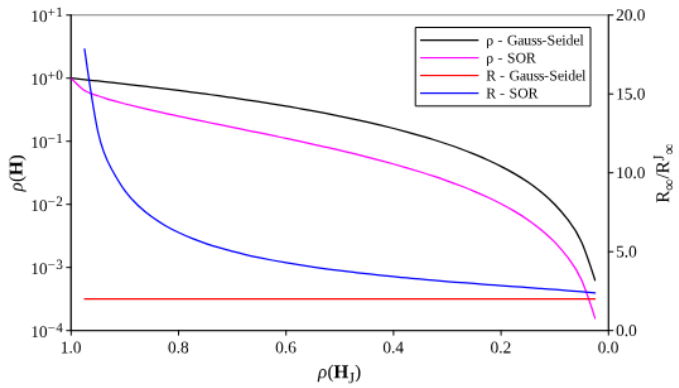
\includegraphics[width=5cm]{img/gs3.png}
	\label{SOR}
	\caption{Gauss-Siedel vs}
\end{figure}
\end{multicols}

\section{Implementazione pratica del metodo SOR}

Riprendendo l'Eq.(11),

\[
\mathbf{\phi}^{(m+1)} = \omega \mathbf{L} \mathbf{\phi}^{(m+1)} + \left[ (1 - \omega) \mathbf{I} + \omega \mathbf{U} \right] \mathbf{\phi}^{(m)} + \omega \mathbf{q},
\]

e riscrivendola in termini di componenti, si ottiene:

\[
\phi_i^{(m+1)} = \omega \sum_{j=1}^{i-1} l_{i,j} \phi_j^{(m+1)} + (1 - \omega) \phi_i^{(m)} + \omega \sum_{j=i+1}^n u_{i,j} \phi_j^{(m)} + \omega q_i\ \ . 
\]

Per un dominio 2D, utilizzando una notazione a doppio indice e introducendo i coefficienti \(W_{i,j}\), \(E_{i,j}\), \(S_{i,j}\), \(N_{i,j}\), si ha:

\[
\begin{aligned}
	\phi_{i,j}^{(m+1)} &= (1 - \omega) \phi_{i,j}^{(m)} + \omega W_{i,j} \phi_{i-1,j}^{(m+1)} + \omega S_{i,j} \phi_{i,j-1}^{(m+1)} \\
	&\quad + \omega E_{i,j} \phi_{i+1,j}^{(m)} + \omega N_{i,j} \phi_{i,j+1}^{(m)} + \omega q_{i,j}. 
\end{aligned}
\]

---

\section{Strategia iterativa Red \& Black}

Sia il metodo di Gauss-Seidel che il metodo SOR possono implementare una strategia di scansione particolare chiamata \textbf{Red \& Black}.

\paragraph{Passo 1: Aggiornamento dei nodi rossi}

In questa fase, vengono aggiornati solo i nodi \textit{rossi}:

\[
\phi_{i,j}^{(m+1)} = W_{i,j} \phi_{i-1,j}^{(m)} + E_{i,j} \phi_{i+1,j}^{(m)} + S_{i,j} \phi_{i,j-1}^{(m)} + N_{i,j} \phi_{i,j+1}^{(m)} + q_{i,j}. 
\]

\paragraph{Passo 2: Aggiornamento dei nodi neri}

In questa fase, vengono aggiornati solo i nodi \textit{neri}:

\[
\phi_{i,j}^{(m+1)} = W_{i,j} \phi_{i-1,j}^{(m+1)} + E_{i,j} \phi_{i+1,j}^{(m+1)} + S_{i,j} \phi_{i,j-1}^{(m+1)} + N_{i,j} \phi_{i,j+1}^{(m+1)} + q_{i,j}. 
\]

Questa strategia consente un trattamento più coerente di ogni nodo, evitando la generazione di componenti asimmetriche spurie nell'errore. Nella valutazione del flusso in ogni nodo, i flussi dei nodi vicini appartengono tutti alla stessa iterazione.

\begin{multicols}{2}
\begin{figure}[H]
	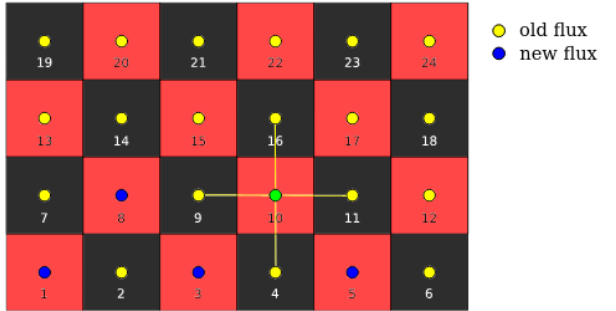
\includegraphics[width=7cm]{img/gs4.png}
	\label{red}
	\caption{step 1 del metodo Red \& Black}
\end{figure}

\begin{figure}[H]
	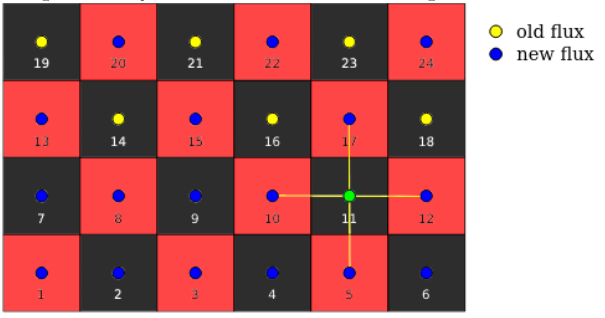
\includegraphics[width=7cm]{img/gs5.png}
	\label{and black}
	\caption{step 2 del metodo Red \& Black}
\end{figure}
\end{multicols}

\section{Metodo Line Overrelaxation (LOR)}

Facciamo riferimento al dominio 2D mostrato in figura. La matrice dei coefficienti \(\mathbf{A}\) del sistema di equazioni nodali può essere letta come una matrice a blocchi (3x3), i cui blocchi diagonali (in blu) sono matrici tridiagonali.

\[
\left[ \begin{array}{l l l l l l l l l}
	a_{11} & a_{12} & 0 & a_{14} & 0 & 0 & 0 & 0 & 0 \\
	a_{21} & a_{22} & a_{23} & 0 & a_{25} & 0 & 0 & 0 & 0 \\
	0 & a_{32} & a_{33} & 0 & 0 & a_{36} & 0 & 0 & 0 \\
	a_{41} & 0 & 0 & a_{44} & a_{45} & 0 & a_{47} & 0 & 0 \\
	0 & a_{52} & 0 & a_{54} & a_{55} & a_{56} & 0 & a_{58} & 0 \\
	0 & 0 & a_{63} & 0 & a_{65} & a_{66} & 0 & 0 & a_{69} \\
	0 & 0 & 0 & a_{74} & 0 & 0 & a_{77} & a_{78} & 0 \\
	0 & 0 & 0 & 0 & a_{85} & 0 & a_{87} & a_{88} & a_{89} \\
	0 & 0 & 0 & 0 & 0 & a_{96} & 0 & a_{98} & a_{99}
\end{array} \right]
\left[ \begin{array}{l}
	\phi_1 \\ \phi_2 \\ \phi_3 \\ \phi_4 \\ \phi_5 \\ \phi_6 \\ \phi_7 \\ \phi_8 \\ \phi_9
\end{array} \right]
=
\left[ \begin{array}{l}
	s_1 \\ s_2 \\ s_3 \\ s_4 \\ s_5 \\ s_6 \\ s_7 \\ s_8 \\ s_9
\end{array} \right]\ \ . 
\]

La matrice può essere riscritta in forma a blocchi:

\[
\left[ \begin{array}{l l l}
	\hat{\mathbf{A}}_{11} & \hat{\mathbf{A}}_{12} & 0 \\
	\hat{\mathbf{A}}_{21} & \hat{\mathbf{A}}_{22} & \hat{\mathbf{A}}_{23} \\
	0 & \hat{\mathbf{A}}_{32} & \hat{\mathbf{A}}_{33}
\end{array} \right]
\left[ \begin{array}{l}
	\hat{\mathbf{\phi}}_1 \\ \hat{\mathbf{\phi}}_2 \\ \hat{\mathbf{\phi}}_3
\end{array} \right]
=
\left[ \begin{array}{l}
	\hat{\mathbf{s}}_1 \\ \hat{\mathbf{s}}_2 \\ \hat{\mathbf{s}}_3
\end{array} \right]\ \ . 
\]

---

\subsubsection{Equazione generica del sistema}

L'equazione generica del sistema (28), scritta in forma a blocchi, è:

\[
\hat{\mathbf{A}}_{i,i-1} \hat{\mathbf{\phi}}_{i-1} + \hat{\mathbf{A}}_{i,i} \hat{\mathbf{\phi}}_i + \hat{\mathbf{A}}_{i,i+1} \hat{\mathbf{\phi}}_{i+1} = \hat{\mathbf{s}}_i\ \ . 
\]

Il primo termine riguarda i flussi della riga \(i-1\), mentre il terzo termine riguarda i flussi della riga \(i+1\). Quando si trattano i nodi della \(i\)-esima riga, quelli sulla riga \(i-1\) sono già stati calcolati. Si può quindi adottare una strategia simile a Gauss-Seidel:

\[
\hat{\mathbf{A}}_{i,i} \hat{\mathbf{\phi}}_i^{(m+1)} = \hat{\mathbf{s}}_i - \hat{\mathbf{A}}_{i,i-1} \hat{\mathbf{\phi}}_{i-1}^{(m+1)} - \hat{\mathbf{A}}_{i,i+1} \hat{\mathbf{\phi}}_{i+1}^{(m)}\ \ . 
\]

L'equazione sopra è un **sistema tridiagonale** che può essere risolto efficientemente con l'algoritmo di Thomas.

---

\subsection*{Introduzione dell'overrelaxation}

Come fatto per il metodo SOR, anche qui possiamo introdurre un'overrelaxation, scrivendo:

\[
\hat{\mathbf{A}}_{i,i} \hat{\mathbf{\phi}}_i^{(m+1)} = \hat{\mathbf{A}}_{i,i} \hat{\mathbf{\phi}}_i^{(m)} + \omega \left[ \hat{\mathbf{A}}_{i,i} \hat{\mathbf{\phi}}_i^{(m+1)} - \hat{\mathbf{A}}_{i,i} \hat{\mathbf{\phi}}_i^{(m)} \right]_{GS}\ \ . 
\]

Grazie all'Eq.(30), possiamo sostituire il primo termine tra parentesi per ottenere:

\[
\hat{\mathbf{A}}_{i,i} \hat{\mathbf{\phi}}_i^{(m+1)} = \omega \hat{\mathbf{s}}_i - \omega \hat{\mathbf{A}}_{i,i-1} \hat{\mathbf{\phi}}_{i-1}^{(m+1)} - \omega \hat{\mathbf{A}}_{i,i+1} \hat{\mathbf{\phi}}_{i+1}^{(m)} + (1 - \omega) \hat{\mathbf{A}}_{i,i} \hat{\mathbf{\phi}}_i^{(m)}\ \ . 
\]

Anche in questo caso, il lato destro è un termine noto, mentre la matrice \(\hat{\mathbf{A}}_{i,i}\) è tridiagonale.

---

\subsection*{Implementazione pratica del metodo LOR}

Con riferimento alla figura precedente e adottando una notazione a doppio indice, possiamo scrivere:

\[
\begin{array}{l}
	W_{i,j} \phi_{i-1,j}^{(m+1)} + O_{i,j} \phi_{i,j}^{(m+1)} + E_{i,j} \phi_{i+1,j}^{(m+1)} = -\omega S_{i,j} \phi_{i,j-1}^{(m+1)} - \omega N_{i,j} \phi_{i,j+1}^{(m)} \\
	\quad + \omega q_{i,j} + (1 - \omega) \left[ W_{i,j} \phi_{i-1,j}^{(m)} + O_{i,j} \phi_{i,j}^{(m)} + E_{i,j} \phi_{i+1,j}^{(m)} \right]\ \ . 
\end{array}
\]

È un'equazione a tre punti. Procedendo per colonne, l'Eq.(33) diventa:

\[
\begin{array}{l}
	S_{i,j} \phi_{i,j-1}^{(m+1)} + O_{i,j} \phi_{i,j}^{(m+1)} + N_{i,j} \phi_{i,j+1}^{(m+1)} = -\omega W_{i,j} \phi_{i-1,j}^{(m+1)} - \omega E_{i,j} \phi_{i+1,j}^{(m)} \\
	\quad + \omega q_{i,j} + (1 - \omega) \left[ S_{i,j} \phi_{i,j-1}^{(m)} + O_{i,j} \phi_{i,j}^{(m)} + N_{i,j} \phi_{i,j+1}^{(m)} \right]\ \ .
\end{array}
\]


\begin{figure}[H]
	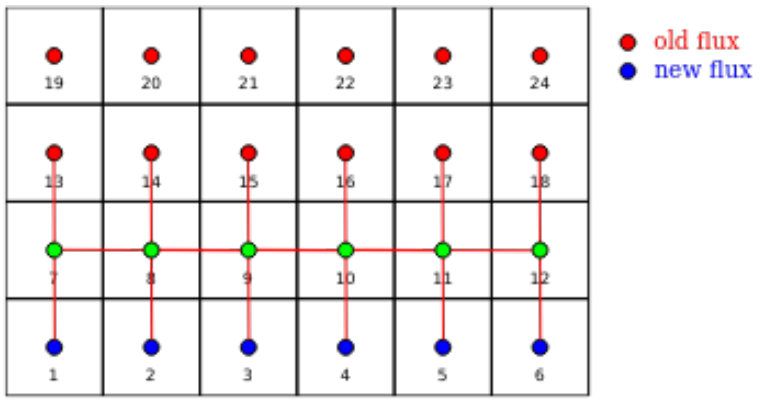
\includegraphics[width=5cm]{img/gs6.png}
	\label{  }
	\caption{  }
\end{figure}